\section{Modeling of Giraf administration}
To model the Giraf administration program a class diagram was made, see Figure \vref{fig:classOversigt}. This give an overview of what we would have to implement in our program and the class diagram describe, how the base model would look like. The Giraf administration needs a user before it can get all the Giraf administration applications that the user can administer. In the model three different persons is important to remember the child and the users who can be either a parent or a kindergarten teacher. The user needs to have a connection with a child and the child's mobile device before the Giraf administration can detect which Giraf mobile applications the device has and then foreach Giraf mobile application finds the Giraf application administrator. The difference on the two Giraf administration applications is that the Giraf application administrator would have a connection to the application on a device e.g. DigiPECS or aSchedule, while User application only is accessible in the Giraf administration.

\begin{figure}[ht]
	\centering
		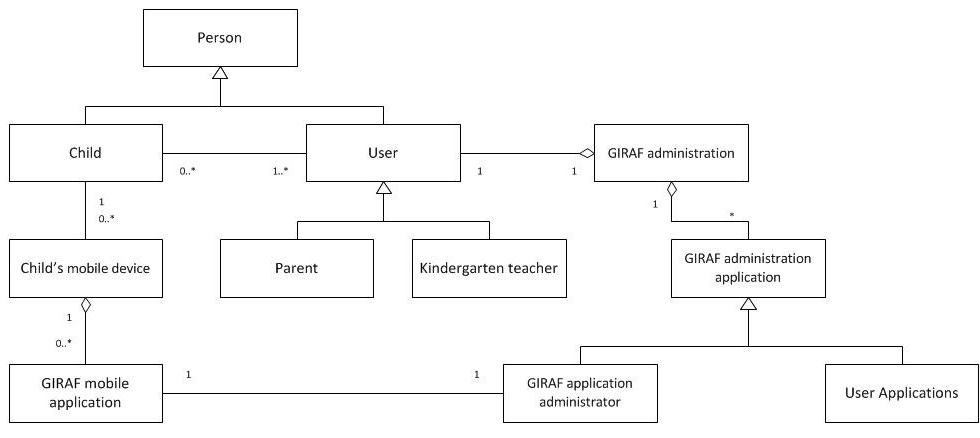
\includegraphics[width=1.00\textwidth]{img/classOversigt.jpg}
	\caption{Giraf administration program}
	\label{fig:classOversigt}
\end{figure}
